%%%%%%
%%%%%%%%%%%%%%%%%%%%%%%%
%
% $Author: Adhiraj Walse $
% $Datum: 2024-2-10  $
%$Pfad:/Documents/ML23-06-Magic-Wand-with-an-Arduino-Nano-33-BLE-sense/Poster/MagicWandtex $
% $Version: 1.0 $
%
%%%%%%%%%%%%%%%%%%%%%%%%



\documentclass[25pt,a0paper, portrait]{tikzposter}
\usepackage[utf8]{inputenc}
\usepackage{xcolor}
\usepackage{graphicx,mwe}
\usepackage{filecontents}
\usepackage{lipsum}
\usepackage{tikz}
\usepackage{multicol}
\usepackage{adjustbox}
\usepackage{blindtext}
\usepackage{comment}

\makeatletter
\def\TP@titlegraphictotitledistance{-6cm}
\settitle{ \centering \vbox{
		\@titlegraphic \\ [\TP@titlegraphictotitledistance] 
		\centering
		\color{titlefgcolor}
		{\bfseries \Huge \sc \@title \par}
		\vspace*{2em}
		{\huge \@author \par}
}}
\makeatother

\setlength{\columnsep}{3cm}

\title{Magic Wand using Arduino Nano BLE 33} 

\author{\textcolor{black}{Adhiraj Walse, Sudeshna Nanda, Srikanth Nanda}}

\titlegraphic{
\includegraphics[height=5.5cm]{images/logo_hs_technik}
\hfill
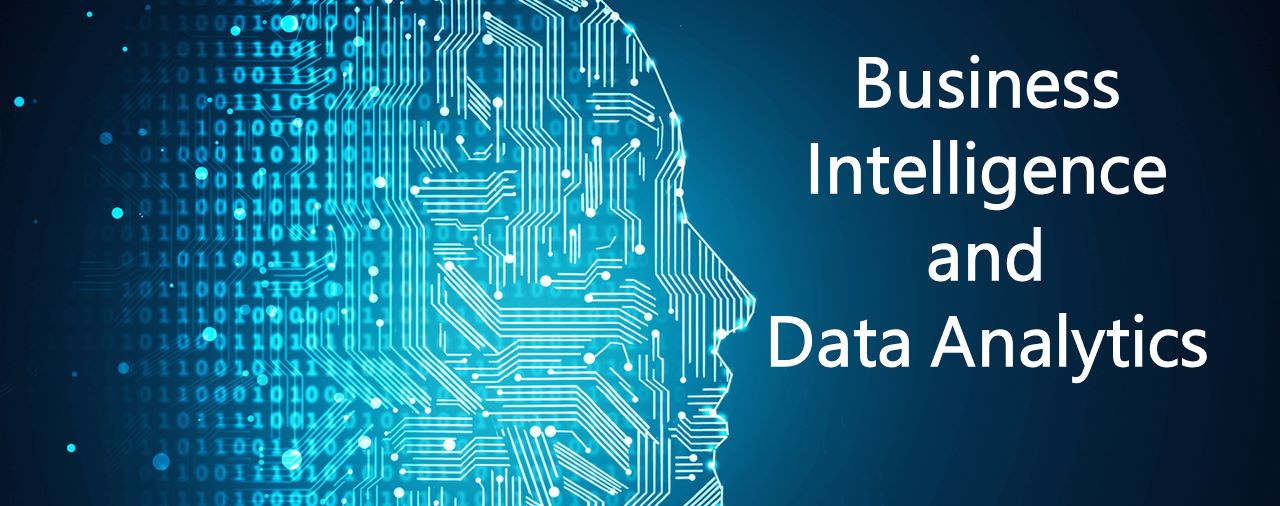
\includegraphics[width=15cm]{images/logo2}
}

\usetheme{Desert}

\begin{document}
	
	\maketitle
	
	\begin{columns} 
		
		\column{0.40}
		{
			\colorlet{blocktitlebgcolor}{blue}
			
			\block{Magic Wand using Arduino 33 BLE Sense}
			{
				The convergence of Machine Learning and the Internet of Things (IoT) has driven remarkable advancements in technology. This project explores the application of Tiny Machine Learning (TinyML) using the Arduino Nano 33 BLE Sense to develop a magic wand capable of gesture recognition.  
				
				The primary focus is on implementing gesture recognition directly on the Arduino Nano 33 BLE Sense, addressing the limitations associated with cloud-based processing. Key challenges include managing memory constraints, ensuring accurate recognition of both predefined and unknown gestures, and reducing false detections. The goal is to develop a TinyML solution that enables real-time, reliable gesture recognition on the magic wand. This project demonstrates the potential of edge-based machine learning on devices with limited resources, paving the way for innovative use cases and applications.
				
				\textbf{Key Features:}
				
				\begin{itemize}
					
					\item Leverages the Arduino Nano 33 BLE Sense equipped with a three-axis accelerometer.
					
					\item Implements a Neural Network model using TensorFlow Lite (TFLite).
					
					\item Detects predefined gestures: wing (W), ring (O), and slope (L).
					
				\end{itemize}
				
			}


			\block{Sensors in Arduino Nano 33 BLE Sense}
			{
				\begin{itemize}
					
					\item \textbf{LSM9DS1} - an Inertial Measurement Unit (IMU) that includes a 3D accelerometer, gyroscope, and magnetometer, enabling detection of orientation, motion, and vibrations.
					
					\item \textbf{MP34DT05} - a microphone capable of capturing and analyzing sound in real time, suitable for creating voice interfaces.
					
					\item \textbf{HTS221} - a sensor that measures relative humidity and temperature.
					
					\item \textbf{LPS22HB} - a sensor designed to read barometric pressure.
					
					\item \textbf{ADPS-9960} - a digital sensor for proximity, ambient light, RGB detection, and gesture recognition.
					
				\end{itemize}
				
			}

			\block{Implementation}
			{
		
				\begin{itemize}			
					
					\item \textbf{Real-Time Hand Movement Detection:}
					
					The magic wand incorporates the Arduino Nano 33 BLE Sense mounted on the end of a stick. Its three-axis accelerometer captures hand movements in real time.
					
					\item \textbf{Integration of TinyML Model:}
					
					The accelerometer data is processed by a deep-learning model implemented using TensorFlow Lite (TFLite), trained to identify specific gestures.
					
					\item \textbf{Gesture-Based Visual Output:}
					
					The Arduino board decodes the recognized gestures and displays corresponding visual feedback on the terminal.
					
				\end{itemize}
				
		}

			
			\block{Future scope}
			{
				
				\begin{itemize}
					
					\item Expanding the model to recognize additional gestures.
					
					\item Utilizing the board's BLE functionality for wireless communication with the computer.
					
					\item Anticipating advancements in TinyML technology to improve the board's performance in the future.
					
					\item Integrating an LED on the wand to light up in response to recognized hand movements.
					
				\end{itemize}
				
			}
	
			\block{Conclusion }
			{	
				The magic wand project leverages Tiny Machine Learning with the Arduino Nano 33 BLE Sense to deliver precise gesture recognition. It reliably identifies predefined gestures—wing, ring, and slope—while effectively managing unknown gestures. This implementation highlights the capabilities of edge-based machine learning in enabling intuitive and interactive applications.
			}

		}
		
		\column{0.60}
		{
			\colorlet{blocktitlebgcolor}{blue}
		
			\block{DataSet}
			{
			
				For our Magic Wand project, a bespoke database was meticulously crafted to cater specifically to our model's unique requirements. The database, stored as a .json file, encapsulates raw accelerometer data obtained from the Arduino Nano 33 BLE Sense board. Each participant in our team, dedicatedly recorded a minimum of 70 trials for the "W," "O," and "L" gestures, ensuring a robust representation of gesture nuances.
				
			    Notably, the dataset's structure accounts for the computer screen size, and each recorded gesture spans a duration of around 2 seconds. This comprehensive and inclusive methodology empowers our model with the depth and breadth required for accurate, efficient, and effective gesture recognition.
		    
			}
	
			\block{Challenges and Solutions}
			{
		
				\begin{enumerate}
					
					\item \textbf{Controlling Data Model Size:}
					
					\begin{itemize}
						
						\item \textbf{Challenge:} The Arduino Nano 33 BLE Sense has limited memory capacity.
						
						\item \textbf{Solution:} Applying optimization techniques, such as model quantization, to minimize the model size while maintaining accuracy.
						
					\end{itemize}
					
					\item \textbf{Training the Model for "Unknown" Gestures:}
					
					\begin{itemize}
						
						\item \textbf{Challenge:} Achieving accurate detection of "unknown" gestures.
						
						\item \textbf{Solution:} Enhancing training with diverse datasets and using methods like transfer learning to improve the model's ability to identify new gestures.
						
					\end{itemize}
					
					\item \textbf{Ensuring Accurate Model Training:}
					
					\begin{itemize}
						
						\item \textbf{Challenge:} Precisely training the TinyML model to recognize predefined gestures.
						
						\item \textbf{Solution:} Conducting iterative training with labeled data, refining model parameters, and validating performance across a wide range of hand movements.
						
					\end{itemize}
					
				\end{enumerate}
			
			}

		\block{Tensorflow Process}
		{
			
			\begin{tikzfigure}
				
				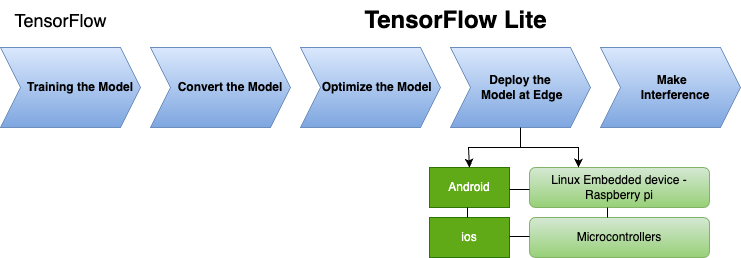
\includegraphics[height= 18 cm , width=43 cm]{images/Tensorflow}
				
			\end{tikzfigure}	
			
			Utilizing TensorFlow’s capabilities, we implement a Convolutional Neural Network (CNN) on the Arduino Nano 33 BLE Sense to enable on-device machine learning. TensorFlow Lite optimizes the model's performance, ensuring efficient execution and real-time gesture recognition without sacrificing speed or accuracy.
		}
		
		\block{Results}
		{
				\begin{tikzfigure}
					
					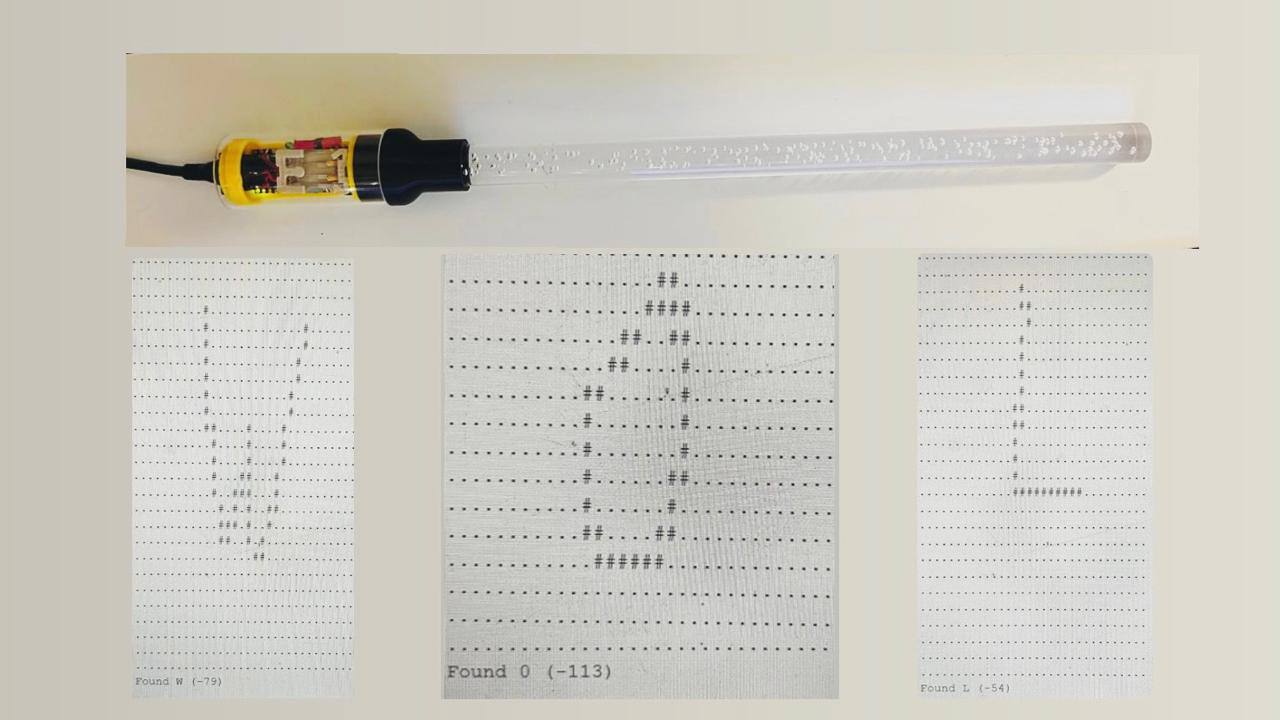
\includegraphics[height= 24 cm, width=\linewidth]{images/output}
						
				\end{tikzfigure}	
		
				\begin{itemize}
					
					\item Accurate Recognition: Consistent and reliable identification of predefined gestures.
					
			\end{itemize}
		}
	}		
		
	\end{columns}
	
\end{document}

